\chapter{Bài 11. Một số lực trong thực tiễn}
\begin{center}
	\textit{(6 tiết)}
\end{center}
\section{MỤC TIÊU DẠY HỌC}
\begin{center}
	\begin{longtable}{|M{2.5cm}|L{12.5cm}|M{2cm}|}
		\hline
		\thead{Biểu hiện\\ năng lực} & \thead{Mục tiêu} & \thead{STT}\\
		\hline
		\multicolumn{3}{|c|}{\textbf{ Năng lực vật lí}}\\
		\hline
		1.1 & Nếu được khái niệm, công thức tính trọng lực. &1 \\
		\hline
		1.4 & Phân biệt được trọng lực và trọng lượng. &2 \\
		\hline
		1.1 & Nếu được khái niệm lực căng dây. &3 \\
		\hline
		1.1 & Nêu được những đặc điểm của lực ma sát nghỉ, ma sát trượt. &4 \\
		\hline
		1.1 & Viết được công thức tính độ lớn của lực ma sát trượt. &5 \\
		\hline
		1.5 & Mô tả được bằng các ví dụ thực tiễn và biểu diễn được lực ma sát. &6 \\
		\hline
			1.5 & Lấy được ví dụ về ích lợi và tác hại của lực ma sát trong đời sống. &7 \\
		\hline
		1.5 & Vận dụng kiến thức lực ma sát để giải thích một số hiện tượng trong thực tế. &8 \\
		\hline
		1.2 & Vận dụng đặc điểm của lực ma sát để giải các bài toán cơ bản. &9 \\
		\hline
		1.2 & Biểu diễn được lực cản, lực nâng trong trường hợp cụ thể.&10 \\
		\hline
		1.2 & Vận dụng đặc điểm của lực cản và lực nâng để giải một số bài toán đơn giản.&11 \\
		\hline
		\multicolumn{3}{|c|}{\textbf{Năng lực chung}}\\
		\hline
		TC - TH& Tích cực thực hiện các nhiệm vụ đặt ra cho nhóm khi tìm hiểu các lực trong thực tiễn.	& 12\\
		\hline
	\end{longtable}
\end{center}
\section{THIẾT BỊ DẠY HỌC VÀ HỌC LIỆU}
\begin{itemize}
	\item Tivi/máy chiếu;
	\item SGK.
\end{itemize}
\section{TIẾN TRÌNH DẠY HỌC}
\subsection{TIẾN TRÌNH}\begin{center}
	\begin{longtable}{|L{2.75cm}|C{1.25cm}|L{5cm}|L{3.5cm}|L{4cm}|}
		\hline
		\thead{Tiến trình} & \thead{Mục\\tiêu} & \thead{Nội dung dạy học \\trọng tâm} & \thead{PP,\\ KTDH} & \thead{Phương pháp \\đánh giá}\\
		\hline
		\textbf{Hoạt động 1:} Tìm hiểu về lực hấp dẫn và trọng lực& 1, 2, 12  & Định luật vạn vật hấp dẫn, khái niệm trọng lực, khái niệm trọng lượng  &PPDH: Thuyết trình  & GV đánh giá dựa trên câu trả lời của HS.\newline
		PP đánh giá: quan sát, nghe.  \\
		\hline
		\textbf{Hoạt động 2:} Tìm hiểu về lực ma sát trượt & 4, 5, 6, 7 & Lực ma sát trượt, biểu thức xác định độ lớn lực ma sát trượt &PPDH: Thuyết trình  & GV đánh giá dựa trên câu trả lời của HS.\newline
		PP đánh giá: quan sát, nghe.  \\
		\hline
		\textbf{Hoạt động 3:} Tìm hiểu về lực ma sát nghỉ và ma sát lăn& 4, 6, 7 & Lực ma sát nghỉ, lực ma sát lăn &PPDH: Thuyết trình  & GV đánh giá dựa trên câu trả lời của HS.\newline
		PP đánh giá: quan sát, nghe.  \\
		\hline
		\textbf{Hoạt động 4:} Vận dụng biểu thức xác định độ lớn lực ma sát trượt để giải các bài toán cơ bản& 5, 9, 12 & Vận dụng biểu thức xác định độ lớn lực ma sát trượt &PPDH: Đàm thoại  & GV đánh giá dựa trên bài tập ví dụ của HS.\newline
		PP đánh giá: quan sát, nghe.  \\
		\hline
		\textbf{Hoạt động 5:} Tìm hiểu về lực căng dây& 3, 12 & Đặc điểm lực căng dây, biểu diễn lực căng dây &PPDH: Thuyết trình  & GV đánh giá dựa trên câu trả lời của HS.\newline
		PP đánh giá: quan sát, nghe.  \\
		\hline
		\textbf{Hoạt động 6:} Tìm hiểu về lực đẩy Archimedes& 10, 11, 12 & Đặc điểm lực đẩy Archimedes &PPDH: Thuyết trình  & GV đánh giá dựa trên câu trả lời của HS.\newline
		PP đánh giá: quan sát, nghe.  \\
		\hline
	\end{longtable}
\end{center}
\subsection{CÁC HOẠT ĐỘNG HỌC}
% ==========================================================================================
\hoatdong
{Tìm hiểu về lực hấp dẫn và trọng lực
}
{\begin{itemize}
		\item HS trình bày được biểu thức định luật vạn vật hấp dẫn.
		\item HS nêu được trọng lực là trường hợp riêng của lực hấp dẫn.
		\item HS phân biệt được trọng lực và trọng lượng.
	\end{itemize}
}
{Câu trả lời của HS cho các câu hỏi gợi mở của GV.
}
{\textit{\underline{* GV chuyển giao nhiệm vụ học tập}}
	\begin{itemize}[label=-]
		\item GV giới thiệu chuyển động của các hành tinh xung quanh Mặt Trời, vệ tinh xung quanh Trái Đất, vật trên Trái Đất khi thả thì rơi xuống đất đều nhờ vào tác dụng của lực hấp dẫn. Mọi vật trong vũ trụ đều đang tương tác với nhau bằng lực hấp dẫn.
		\begin{center}
			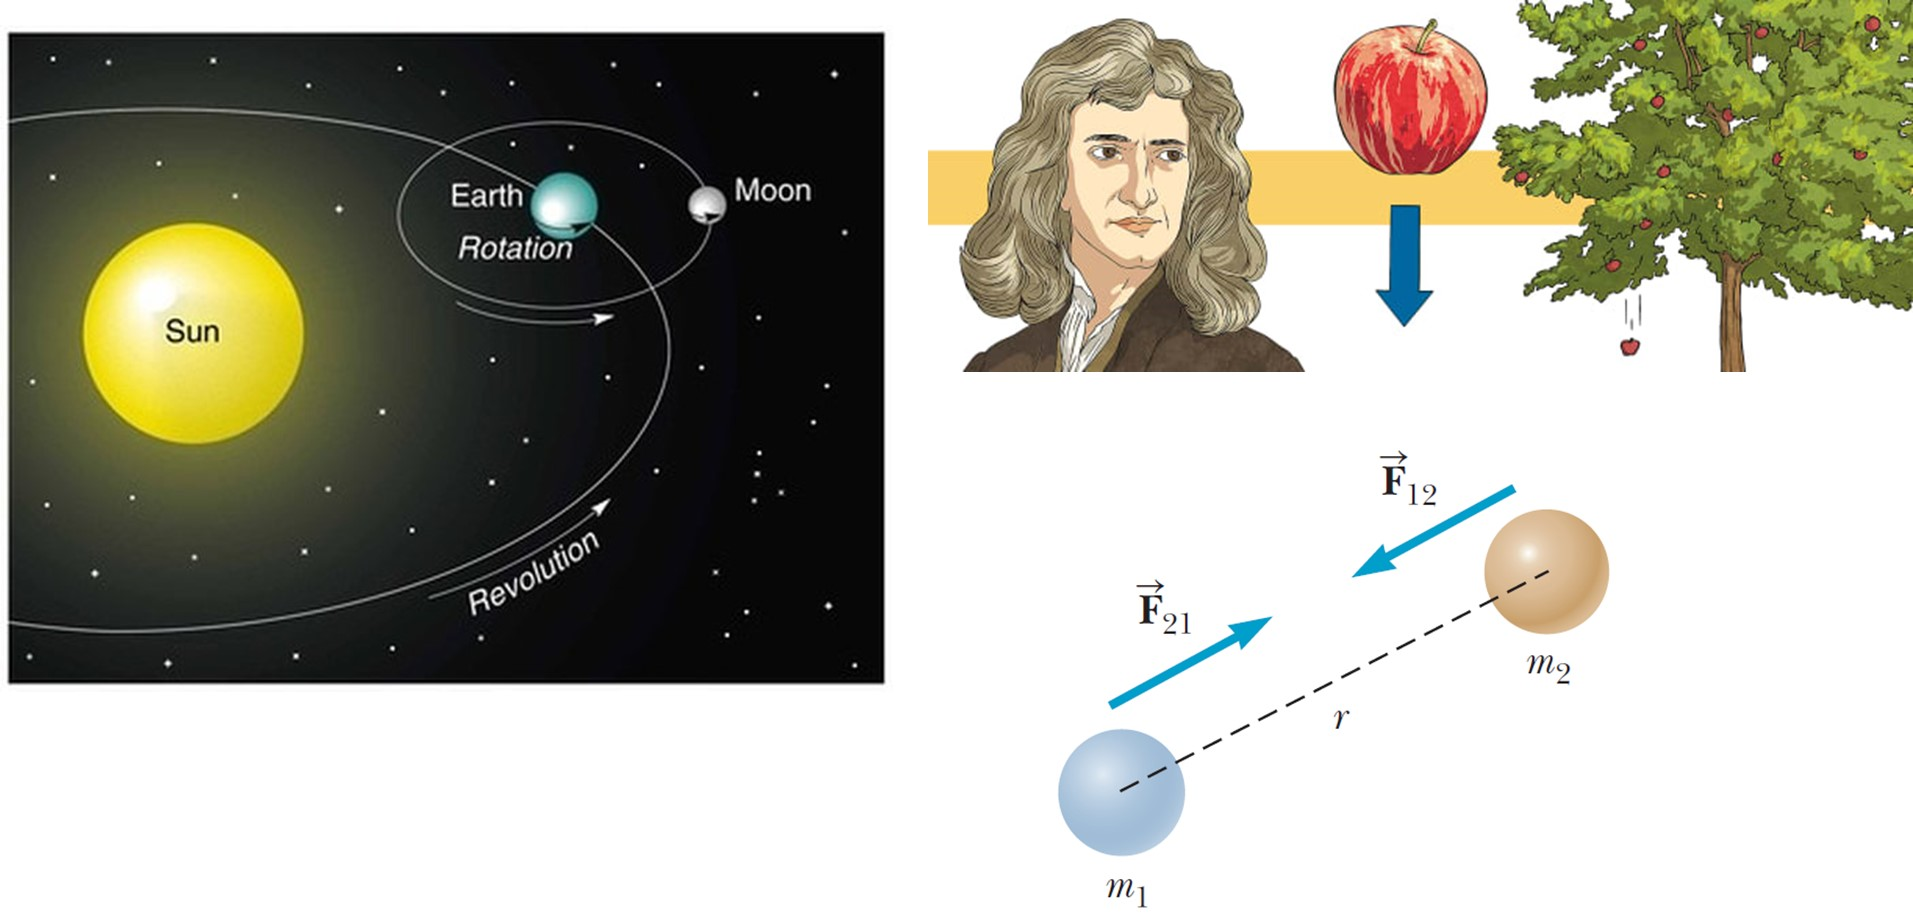
\includegraphics[scale=0.4]{figs/G10-BAI11-1}
		\end{center}
		\item GV giới thiệu cho HS về định luật vạn vật hấp dẫn.
		\item GV giới thiệu cho HS về giới hạn sử dụng định luật vạn vật hấp dẫn:
		\begin{itemize}[label=$\bullet$]
			\item Định luật áp dụng với trường hợp khoảng cách giữa các vật rất lớn so với kích thước giữa chúng (chất điểm).
			\item Hai vật đồng chất, hình cầu thì $r$ là khoảng cách nối tâm 2 vật. Lực hấp dẫn trùng phương nối tâm và có điểm đặt tại tâm mỗi vật.
		\end{itemize}
		\item GV giới thiệu cho HS trọng lực là trường hợp riêng của lực hấp dẫn. Từ đó, GV hướng dẫn HS xây dựng biểu thức gia tốc trọng trường.
		\item GV đặt câu hỏi: \textit{"Dựa vào biểu thức gia tốc trọng trường em hãy cho biết gia tốc trọng trường phụ thuộc vào các yếu tố nào?"}
		\item GV giới thiệu cho HS khái niệm trọng lượng: Trọng lượng là số chỉ của dụng cụ đo (dụng cụ xác định trọng lực hoặc khối lượng). Trong một số tình huống, trọng lực và trọng lượng có giá trị khác nhau.
		\item GV yêu cầu HS thực hiện ví dụ 1.
	\end{itemize}
		\textit{\underline{* HS thực hiện nhiệm vụ học tập}}
	\begin{itemize}[label=-]
		\item HS chú ý lắng nghe, đặt câu hỏi.
		\item HS hoạt động cá nhận để thực hiện ví dụ 1.
	\end{itemize}
	\textit{\underline{* HS báo cáo kết quả nhiệm vụ học tập}}
	\begin{itemize}[label=-]
		\item GV mời 1 HS lên bảng trình bày kết quả ví dụ 1.
		\item Các HS khác theo dõi và nhận xét.
		\item GV chỉnh lí và hợp thức hóa kiến thức.
	\end{itemize}
}
% ==========================================================================================
\hoatdong
{Tìm hiểu về lực ma sát trượt.
}
{\begin{itemize}
		\item HS trình bày được đặc điểm của lực ma sát trượt.
		\item HS viết được biểu thức xác định độ lớn của lực ma sát trượt.
	\end{itemize}
}
{Kết quả báo cáo thí nghiệm của các nhóm HS.
}
{	\textit{\underline{GV chuyển giao nhiệm vụ học tập}}
	\begin{itemize}[label=-]
		\item GV đặt câu hỏi gợi mở vấn đề: Trong các trường hợp phanh xe gấp, bánh xe sẽ để lại vết trượt đen dài trên đường. Điều này là do đâu?
		\begin{center}
			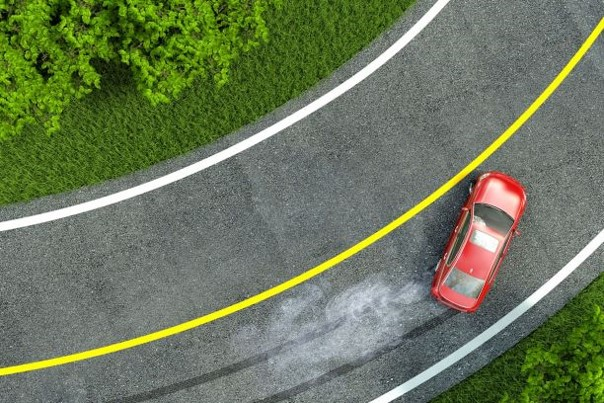
\includegraphics[scale=0.4]{figs/G10-BAI11-2}
		\end{center}
		\item GV giới thiệu cho HS bản chất của lực ma sát trượt là do lực tương tác tĩnh điện giữa 2 bề mặt tiếp xúc khi cọ xát với nhau.
		\begin{center}
			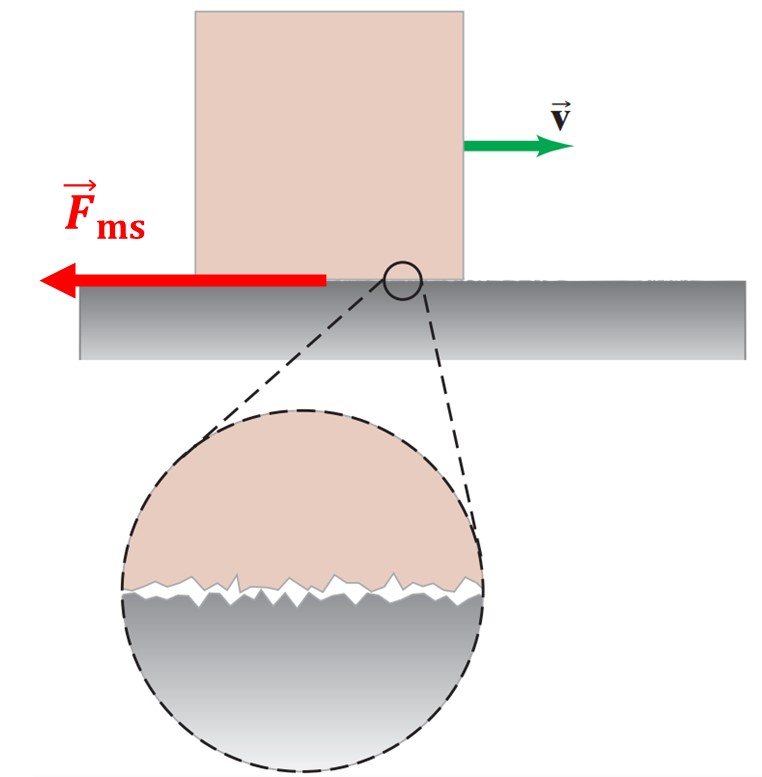
\includegraphics[scale=0.5]{figs/G10-BAI11-3}
		\end{center}
		\item Dựa vào kiến thức về tương tác tĩnh điện mà HS đã học ở chương trình KHTN, GV yêu cầu HS dự đoán về hướng của lực ma sát trượt.
		\item GV chia lớp thành 6 nhóm và giao cho các nhóm thực hiện 2 thí nghiệm sau (Nhóm 1, 2, 3 thực hiện thí nghiệm 1 và Nhóm 4, 5, 6 thực hiện thí nghiệm 2):
		\begin{itemize}[label=$\bullet$]
			\item \textbf{THÍ NGHIỆM 1:} \textit{Khảo sát sự phụ thuộc của lực ma sát vào vật liệu và tình trạng bề mặt tiếp xúc.}\\
			\textbf{\textit{Dụng cụ:}} Lực kế (có GHĐ \SI{1.0}{\newton} và ĐCNN \SI{0.01}{\newton}), khối gỗ hình hộp chữ nhật, các bề mặt: gỗ, giấy, inox.\\
			\textbf{\textit{Tiến hành:}}
			\begin{center}
				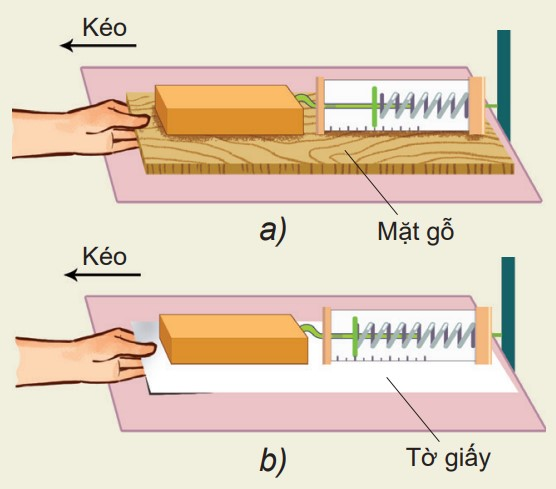
\includegraphics[scale=0.7]{figs/G10-BAI11-4.jpg}
			\end{center}
			\begin{itemize}
				\item Gắn lực kế vào giá thí nghiệm để cố định lực kế theo phương nằm ngang.
				\item Móc khối gỗ vào lực kế, lần lượt kéo các mặt tiếp xúc (mặt gỗ, mặt tờ giấy, mặt inox) theo phương nằm ngang để chúng trượt đều dưới khối gỗ.
				\item Ghi số chỉ của lực kế vào bảng bên dưới. Lấy giá trị trung bình của các số chỉ lực kế làm độ lớn của lực ma sát trượt.
				\begin{center}
					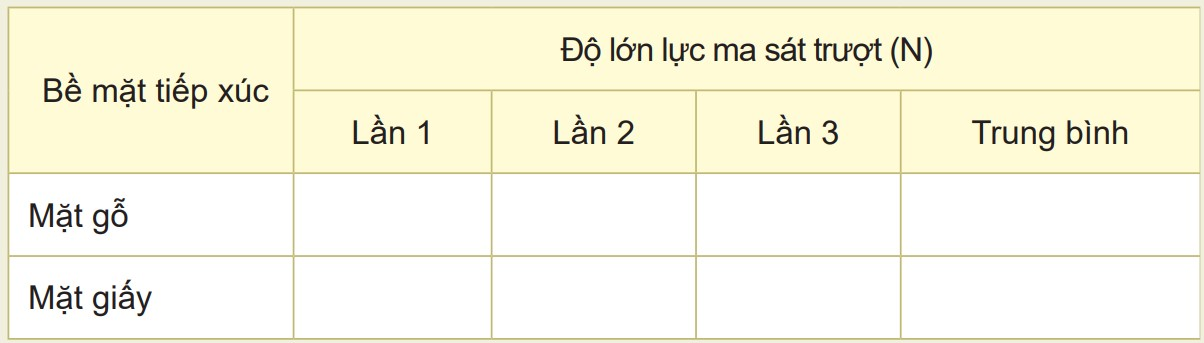
\includegraphics[scale=0.55]{figs/G10-BAI11-5}
				\end{center}
			\end{itemize}
				\textbf{\textit{Thảo luận và phân tích:}}
				\begin{itemize}
					\item Nêu các lực tác dụng lên khối gỗ khi mặt tiếp xúc bên dưới nó được kéo trượt đều. Tại sao khi đó số chỉ của lực kế bằng độ lớn của lực ma sát trượt?
					\item Sắp xếp thứ tự theo mức tăng dần lực ma sát trên mỗi bề mặt.
				\end{itemize}
			\item \textbf{THÍ NGHIỆM 2:} \textit{Khảo sát mối liên hệ giữa độ lớn của lực ma sát trượt với độ lớn của áp lực lên bề mặt tiếp xúc.}\\
			\textbf{\textit{Dụng cụ:}} Lực kế (có GHĐ \SI{1.0}{\newton} và ĐCNN \SI{0.01}{\newton}), ba khối gỗ hình hộp chữ nhật giống nhau, mặt tiếp xúc: gỗ.\\
			\textbf{\textit{Tiến hành:}}
			\begin{itemize}
				\item Đo trọng lượng của khối gỗ bằng lực kế.
				\item Gắn lực kế vào giá thí nghiệm để cố định lực kế theo phương nằm ngang.
				\item Móc khối gỗ vào lực kế, kéo mặt tiếp xúc (mặt gỗ) theo phương nằm ngang để nó trượt đều dưới khối gỗ. Ghi lại số chỉ của lực kế trong 3 lần thí nghiệm vào bảng bên dưới. Lấy giá trị trung bình các kết quả đo.
				\item Lần lượt đặt thêm 1, 2 khối gỗ lên trên khối gỗ đầu tiên và lặp lại bước 3.
				\begin{center}
					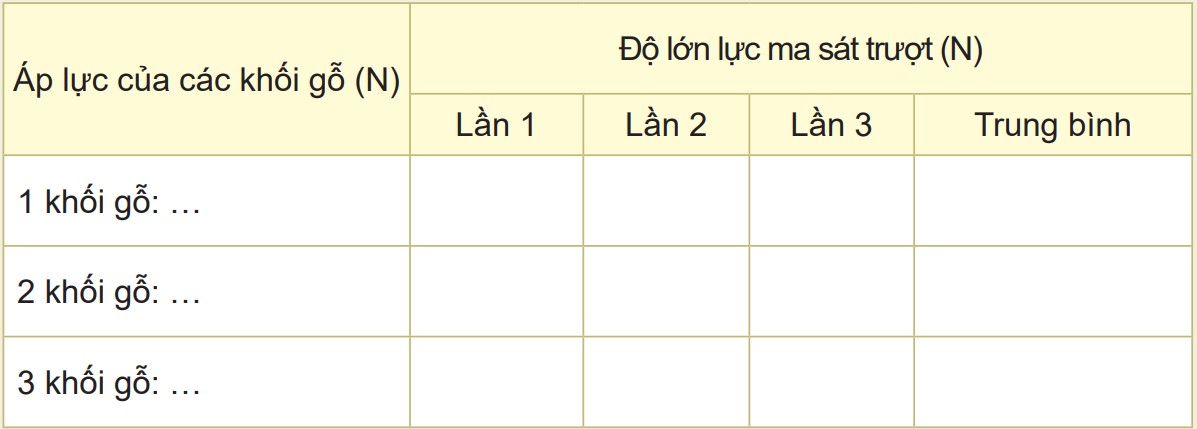
\includegraphics[scale=0.5]{figs/G10-BAI11-6}
				\end{center}
			\end{itemize}
			\textbf{\textit{Thảo luận và phân tích:}}
			\begin{itemize}
				\item Điều gì xảy ra với độ lớn của lực ma sát trượt khi tăng áp lực lên bề mặt tiếp xúc?
				\item Vẽ đồ thị cho thấy sự thay đổi độ lớn của lực ma sát trượt khi tăng dần độ lớn của áp lực.
			\end{itemize}
		\end{itemize}
		\item GV theo dõi, hỗ trợ HS trong quá trình các nhóm thực hiện thí nghiệm.
		
	\end{itemize}
	\textit{\underline{* HS thực hiện nhiệm vụ học tập}}
	\begin{itemize}[label=-]
		\item HS chú ý lắng nghe.
		\item HS hoạt động theo nhóm để thực hiện thí nghiệm.
	\end{itemize}
	\textit{\underline{* HS báo cáo kết quả nhiệm vụ học tập}}
	\begin{itemize}[label=-]
		\item Các nhóm nộp lại báo cáo thí nghiệm cho GV.
		\item GV mời đại diện 2 nhóm HS (2 nhóm thực hiện 2 thí nghiệm độc lập) báo cáo kết quả thí nghiệm của nhóm.
		\item GV yêu cầu HS kết luận về những đặc điểm về độ lớn của lực ma sát trượt.
		\item GV nhận xét, chuẩn hóa kiến thức.
	\end{itemize}
}
